\documentclass{beamer}
\usepackage{graphicx}
\usepackage{verbatim}
\usepackage{amsmath}
\usepackage{amsfonts}
\usepackage{setspace}
% \usepackage{beamerthemesplit} // Activate for custom appearance

\title{Linear Regression Models\\W4315}
\author{Instructor: Dr. Frank Wood}

\date{Required Text: Applied Linear Regression\\
Authors: Kutner, Nachtsheim, Neter}



\DeclareMathOperator*{\Ave}{\mathbb{E}}
\DeclareMathOperator*{\Var}{Var}

\begin{document}

\frame{\titlepage}


\frame[t] {
 \frametitle{Not Registered Yet?}
Fill out the form at\\
http://tinyurl.com/mqfq95
\bigskip

Additional books we will draw material from in this course:
\begin{itemize}
\item Pattern Recognition and Machine Learning, by Christopher M. Bishop. Springer, 2006.
\item Bayesian Data Analysis, Second Edition, by Andrew Gelman, John B. Carlin, Hal S. Stern, and Donald B. Rubin, Chapman \& Hall/CRC Texts in Statistical Science
\end{itemize}




}

\frame[t] {
 \frametitle{Course Description}
Theory and practice of regression analysis, Simple and multiple
regression, including testing, estimation, and confidence
procedures, modeling, regression diagnostics and plots, polynomial
regression, colinearity and confounding, model selection, geometry
of least squares. Extensive use of the computer to analyze data.}

\frame[t] {
 \frametitle{Philosophy and Style}
\begin{itemize}
\item Easy first half.
\item Very hard second half.
\item Frequent, long digressions from the required book.
\item Understanding == proof (derivation) {\em plus} implementation.
\item Practice makes perfect.
\item Frequentist and Bayesian perspectives taught.
\end{itemize}
}


\frame[t] {
 \frametitle{About me}
\begin{itemize}
\item Computer Science PhD, 2007, Brown University
\item Postdoc in Machine Learning, Gatsby Unit, University College London
\item Sports gambling consulting.
\item Former entrepreneur.
\end{itemize}
My research
\begin{itemize}
\item Inference for nonparametric Bayesian models.
\item Compression.
\item Natural language data  modeling.
\end{itemize}
}


\frame[t] {
 \frametitle{Course Outline}
 First half of the course is on the traditional view of linear regression.  The first half of the first half is a formal, theoretical review of single variable regression and its classical, frequentist treatment.

 \begin{itemize}
 \item Roughly 1 chapter per week
 \item 3-5 weeks, linear regression
 \begin{itemize}
 \item Least squares
 \item Maximum likelihood, normal model
 \item Tests / inferences
 \item ANOVA
 \item Diagnostics
 \item Remedial Measures
 \item Linear algebra review
 \item Matrix approach to linear regression
\end{itemize}
\end{itemize}
}


\frame[t] {

The second half of the first half covers multiple regression and the various topics that arise from including multiple predictor variables into models.

 \frametitle{Course Outline Continued}
 \begin{itemize}
 \item 3-4 weeks multiple regression
 \begin{itemize}
 \item Multiple predictor variables
 \item Diagnostics
 \item Tests
 \end{itemize}
 \end{itemize}
 Midterm

}


\frame[t] {

The remainder of the course will deviate from the book and may be ordered differently than what is shown here.  In general we will retain a focus on models that are linear in the parameters, but will look at nonlinear models and Bayesian treatments of linear models.

 \frametitle{Course Outline Continued}
 \begin{itemize}
 \item 3-4 weeks on generalized regression
 \begin{itemize}
 \item Polynomial regression
 \item Logistic regression
 \item Neural networks
 \item Generalized linear models
 \end{itemize}
 \end{itemize}
 \begin{itemize}
 \item 3-4 weeks on Bayesian regression
 \begin{itemize}
 \item MCMC
 \item Bayesian linear regression
 \item Gaussian process regression
 \item Projects
 \end{itemize}
 \end{itemize}
}


\frame[t] {
 \frametitle{Requirements}
 \begin{itemize}
 \item Calculus
 \begin{itemize}
 \item Derivatives, gradients, convexity
 \end{itemize}
 \end{itemize}
 \begin{itemize}
 \item Linear algebra
 \begin{itemize}
 \item Matrix notation, inversion, eigenvectors, eigenvalues, rank, quadratic forms
 \end{itemize}
 \end{itemize}
 \begin{itemize}
 \item Probability
 \begin{itemize}
 \item Random variables
 \item Bayes Rule
 \end{itemize}
 \end{itemize}
 \begin{itemize}
 \item Statistics
 \begin{itemize}
 \item Expectation, variance
 \item Estimation
 \item Bias/Variance
 \item Basic probability distributions
 \end{itemize}
 \end{itemize}
 \begin{itemize}
 \item Programming
 \end{itemize}

}


\frame[t] {
 \frametitle{Projects (homework and final)}
 \begin{itemize}
 \item Software

 \begin{itemize}
 \item For homework -- Matlab.
 \item For final project, don't care:
 \begin{itemize}
 \item R
 \item Matlab
 \item S-Plus
 \item SAS
 \item Minitab
 \item Excel
 \item java, c++, c, assembly, $\ldots$
 \end{itemize}
 \end{itemize}
 \end{itemize}

}

\frame[t] {
 \frametitle{Grading}
 \begin{itemize}
 \item Bi-weekly homework $(35\%)$
 \begin{itemize}
 \item Due every other week
 \begin{itemize}
 \item no late homework accepted
 \end{itemize}
 \item One allowed to be missed
 \item Completing all is ``extra-credit''
 \end{itemize}
  \end{itemize}
 \begin{itemize}
 \item Participation $(5\%)$
 \item Midterm examination $(25\%)$
 \item Final project $(35\%)$
 \item Curve
 \end{itemize}

}

\frame[t] {
 \frametitle{Office Hours / Website}
 \begin{itemize}
 \item $http://www.stat.columbia.edu/\sim fwood$
 \item Office hours : Thursday 7:30-9pm subject to change
 \item Office : Room 1011
 \item TA : Heng
 \begin{itemize}
 \item TA office hours TBD
 \end{itemize}
 \end{itemize}
}

\frame[t] {
 \frametitle{Why regression?}
 \begin{itemize}
 \item Want to model a functional relationship between an ``predictor variable'' (input, independent variable, etc.)
      and a ``response variable'' (output, dependent variable, etc.)
 \begin{itemize}
 \item Examples?
 \end{itemize}
 \end{itemize}
 \begin{itemize}
 \item But real world is noisy, no $f = ma$
 \begin{itemize}
 \item Observation noise
 \item Process noise
 \end{itemize}
 \item Two distinct goals
 \begin{itemize}
 \item Tests about natural of relationship between predictor variables and response variables
 \item Prediction
 \end{itemize}
 \end{itemize}
}

\frame[t] {
 \frametitle{History}
 \begin{itemize}
 \item Sir Francis Galton, $19^{th}$ century
 \begin{itemize}
 \item Studied the relation between heights of parents and children and noted that the children ``regressed'' to the population mean
 \end{itemize}
 \end{itemize}
 \begin{itemize}
 \item ``Regression'' stuck as the term to describe statistical relations between variables
 \end{itemize}
}

\frame[t] {
 \frametitle{Example Applications}
 Trend lines, eg. Google over 6 mo.
\begin{figure}
  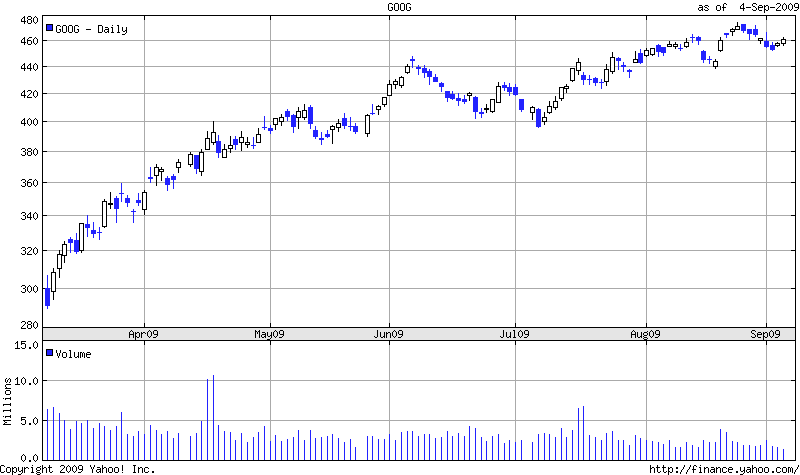
\includegraphics[height=60mm]{google.png}
\end{figure}
}

\frame[t] {
 \frametitle{Others}
 \begin{itemize}
 \item Epidemiology
 \begin{itemize}
 \item Relating lifespan to obesity or smoking habits etc.
 \end{itemize}
 \end{itemize}
 \begin{itemize}
 \item Science and engineering
 \begin{itemize}
 \item Relating physical inputs to physical outputs in complex systems
 \end{itemize}
 \end{itemize}
 \begin{itemize}
 \item Grander

 \begin{center}
 \begin{figure}
  \hspace{-2cm}
  
\includegraphics[height=20mm]{brain.png}
\end{figure}
\end{center}
 \end{itemize}
}

\frame[t] {
 \frametitle{Aims for the course}
\begin{itemize}
\item Given something you would like to predict and some number of covariates
\begin{itemize}
\item What kind of model should you use?
\item Which variables should you include?
\item Which transformations of variables and interaction terms should you use?
\end{itemize}
\item Given a model and some data
\begin{itemize}
\item How do you fit the model to the data?
\item How do you express confidence in the values of the model parameters?
\item How do you regularize the model to avoid over-fitting and other related issues?
\end{itemize}
\end{itemize}

}

\end{document}
